%\begin{figure}
	\begin{center}
		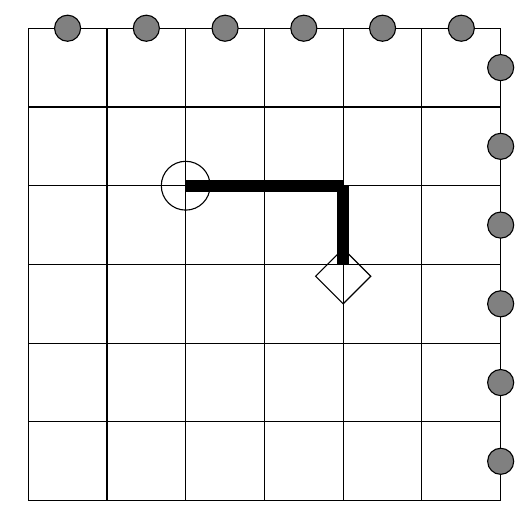
\begin{tikzpicture}
			
			
			
			% Draw solid grid and nodes with circles in the middle of each side
			\draw[step=1cm] (-3,-3) grid (3,3);
			\foreach \i in {-2.5,...,2.5}
			{
				\foreach \j in {-2.5,...,2.5}
				{
					
					
					\begin{scope}[transform canvas={xshift=\i cm,yshift=\j cm}]
						
						\node[right,xshift=0.2cm,yshift=0.4cm] {};
						% Convert \j and \i to integers
						\pgfmathtruncatemacro{\intj}{\j}
						\pgfmathtruncatemacro{\inti}{\i}
						
						\ifnum\intj=2
						\draw node[draw,circle,fill=gray] at (0,0.5) {};
						\fi
						
						\ifnum\inti=2
						\draw node[draw,circle,fill=gray] at (0.5,0) {};
						\fi
						
						
						
						\ifnum\intj=1
						\ifnum \inti=0
						\draw node[label=south:\textbf{}] at (-0.5,0) {};
						\draw node[label=center:\textbf{}] at (0.5,0) {};
						\else
						\ifnum \inti>1
						\draw node[label=center:\textbf{}] at (-0.5,-0.5) {};
						\fi
						\ifnum \inti<1
						\draw node[label=center:\textbf{}] at (-0.5,-0.5) {};
						\fi
						\fi
						\else
						\draw node[label=center:\textbf{}] at (-0.5,-0.5) {};
						\fi
						
					\end{scope}
				}
			}
			
		
	
			
		
			
			\foreach \i in {1,...,1}
			{
				
				\draw[black, line width=1.5mm] (\i,1) -- (\i, 0 );
				
			}
			\foreach \j in {1,...,1}
			{
				
				\draw[black, line width=1.5mm] (-1, \j) -- (1, \j);
				
			}
			
			\def\radius{0.3}
			\draw (-1,1) circle (\radius 1cm);
			
			\def\side{0.7}
			\draw (1,-0.5) -- ++(\side/2,\side/2) -- ++(-\side/2,\side/2) -- ++(-\side/2,-\side/2) -- ++(\side/2,-\side/2) -- cycle;
			
		\end{tikzpicture}
	\end{center}
	
	%\caption{Worm string of adjacent edges. The head is represented with a rhombus, while the tail is represented with a circle. The worm body is highlighted in black as to indicate that it could be formed by ocupied edges if and only if there was no previously occupied edge before. Otherwise it would have been flipped to unoccupied. Notice that this picture is only for the sake of exemplyification, therefore the eigenvalues are omitted.}
	%\label{fig:worm}
	%end{figure}
